\documentclass[final,hyperref={pdfpagelabels=false}, xcolor=dvipsnames]{beamer}
%\mode<presentation>{\usetheme{ZH}}
\mode<presentation>{\usetheme{confposter}}
\usepackage{times}
\usepackage{ragged2e} %% justify the text.
\usepackage{amssymb,amsfonts,amsmath,mathtext,cite,enumerate,float} 
\boldmath
\usepackage[utf8]{inputenc}
\usepackage[english]{babel}
\usepackage{graphicx}
\usepackage{wrapfig}
\usepackage{multirow}
\graphicspath{{figures/}}

\usepackage[orientation=portrait,size=a0,scale=1.]{beamerposter}

%-- Header and footer information ----------------------------------
\newcommand{\footleft}{Laboratory of High Energy Physics, Joint Institute for Nuclear Research, Dubna, Russia}
\newcommand{\footright}{email: pavel.batyuk@jinr.ru}
\title{ Correlation femtoscopy studies at NICA and STAR energies within a viscous hydrodynamic + cascade model vHLLE+UrQMD (Phys.Rev. C96 (2017) no.2, 024911)}
\author{\textit{\underline{P. Batyuk}, Iu. Karpenko, R. Lednicky, L. Malinina, K. Mikhaylov, O. Rogachevsky, D. Wielanek}}
\institute{VBLHEP, JINR, pavel.batyuk@jinr.ru}
%-------------------------------------------------------------------
\setbeamertemplate{headline}{
 \leavevmode
  \begin{columns}
   \column{.05\textwidth}
   
\includegraphics[scale=.5]{NICA_Logo.png}
   %\end{column}
   \column{.75\textwidth}
    \vskip1cm
    \centering
    \usebeamercolor{title in headline}{\color{jblue}\Huge{\textbf{\inserttitle}}\\[0.2ex]}
    \usebeamercolor{author in headline}{\color{fg}\Large{\insertauthor}\\[1ex]}
    \usebeamercolor{institute in headline}{\color{fg}\large{\insertinstitute}\\[1ex]}
    %\vskip1cm
   %\end{column}
   \column{.1\textwidth}
    
\includegraphics[scale=0.3]{vblhep_.png}
  % \end{column}
  %\vspace{1cm}
  \end{columns}
 \vspace{0.5in}
 \hspace{0.5in}\begin{beamercolorbox}[wd=47in,colsep=0.15cm]{cboxb}\end{beamercolorbox}
 \vspace{0.1in}
}
%-- Main Document --------------------------------------------------
\begin{document}
 \begin{frame}[shrink=30]
 \bf
 %%% First part used to formulate a problem to be considered ....
 
 \begin{columns}[t]
 \column{.44\textwidth}
 \begin{block}{Motivation}
 \begin{figure}[T]
    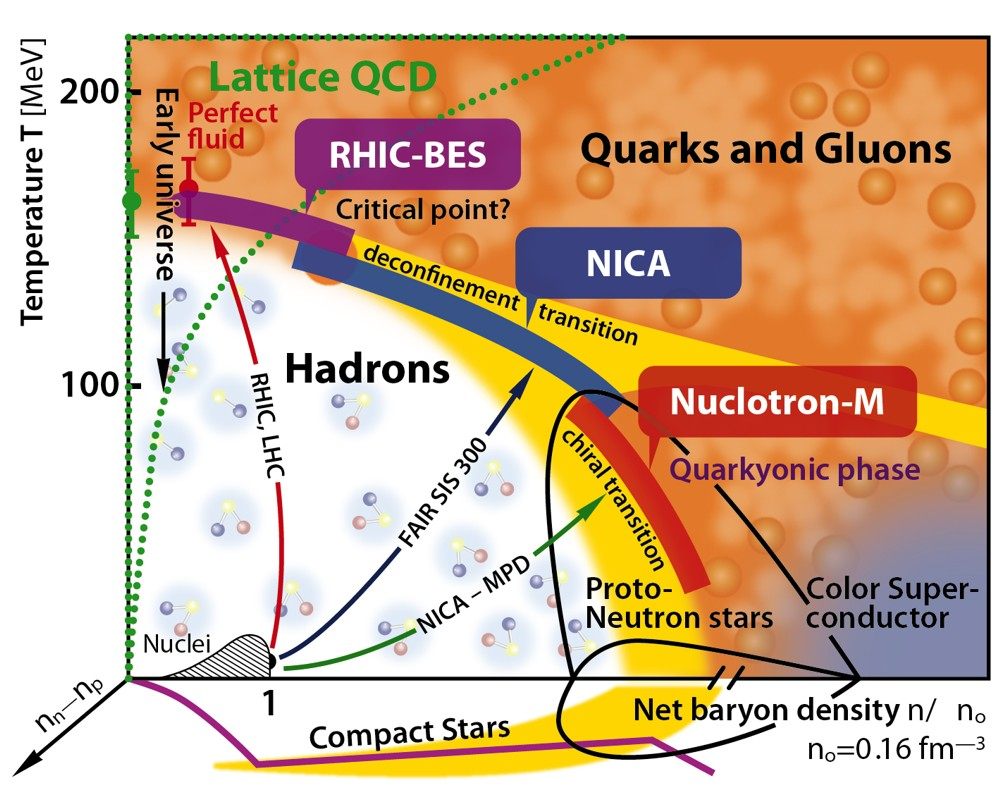
\includegraphics[width=1.\linewidth]{phase.jpg}
 \end{figure}
 \begin{block}{T and $\mu$ at different energies:}
 \begin{itemize}
  \item {\bf RHIC}: $\sqrt{s_{NN}}$ = 62.4, 200 GeV ({\color{red} large T \& small $\mu_{b}$. Smooth, rapid crossover})
  \item {\bf RHIC BES: $\sqrt{s_{NN}}$ = 7.7, 11.5, 19.6, 27, 39 GeV ({\color{red} small T \& moderate $\mu_{b}$. 
  Search for ``critical point''})}
  \item {\bf NICA: $\sqrt{s_{NN}}$ = 4 - 11 GeV ({\color{red} small T \& large $\mu_{b}$}})
  \end{itemize}
 \end{block}
  \end{block}
  
   \begin{block}{Correlation functions from the model}
    \begin{columns}[t]
    \column{.46\textwidth}
   \begin{figure}[H]
           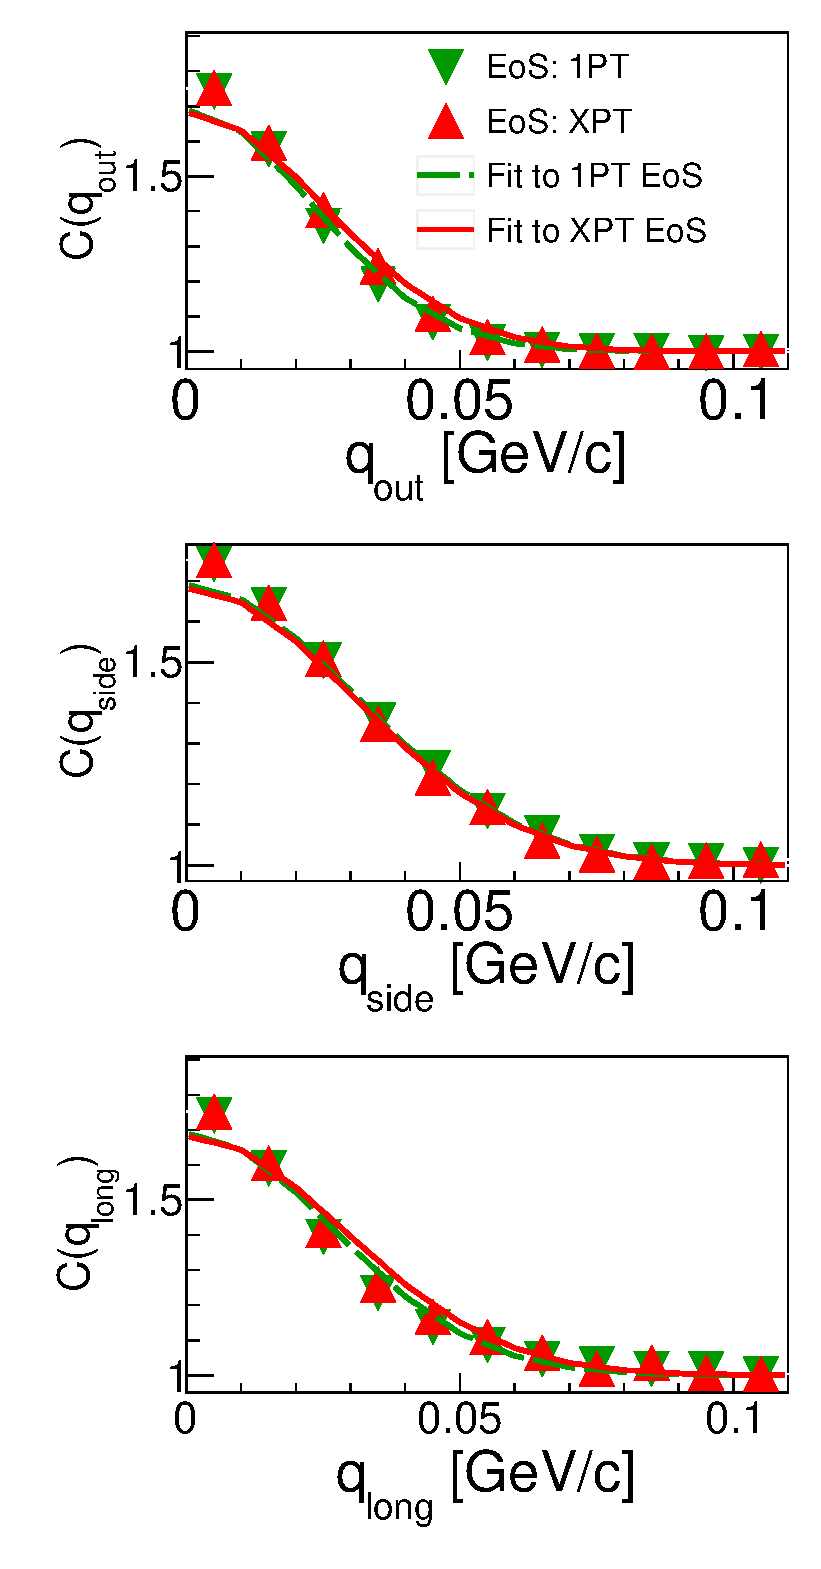
\includegraphics[width=0.99\linewidth]{fig2_poster.eps}
          \caption{1D projections of 3D correlation function 
    of non-interacting identical pion pairs onto ``out'', ``side'' and ``long'' directions.  
   %While projecting onto a direction, other two directions are required to be within the range of (-0.03, 0.03) GeV/c. 
   A fit with the Gaussian function is presented by dashed and solid lines for the 1PT and XPT scenarios, respectively.}
      \end{figure}
    \column{.46\textwidth}
     \begin{figure}[H]
         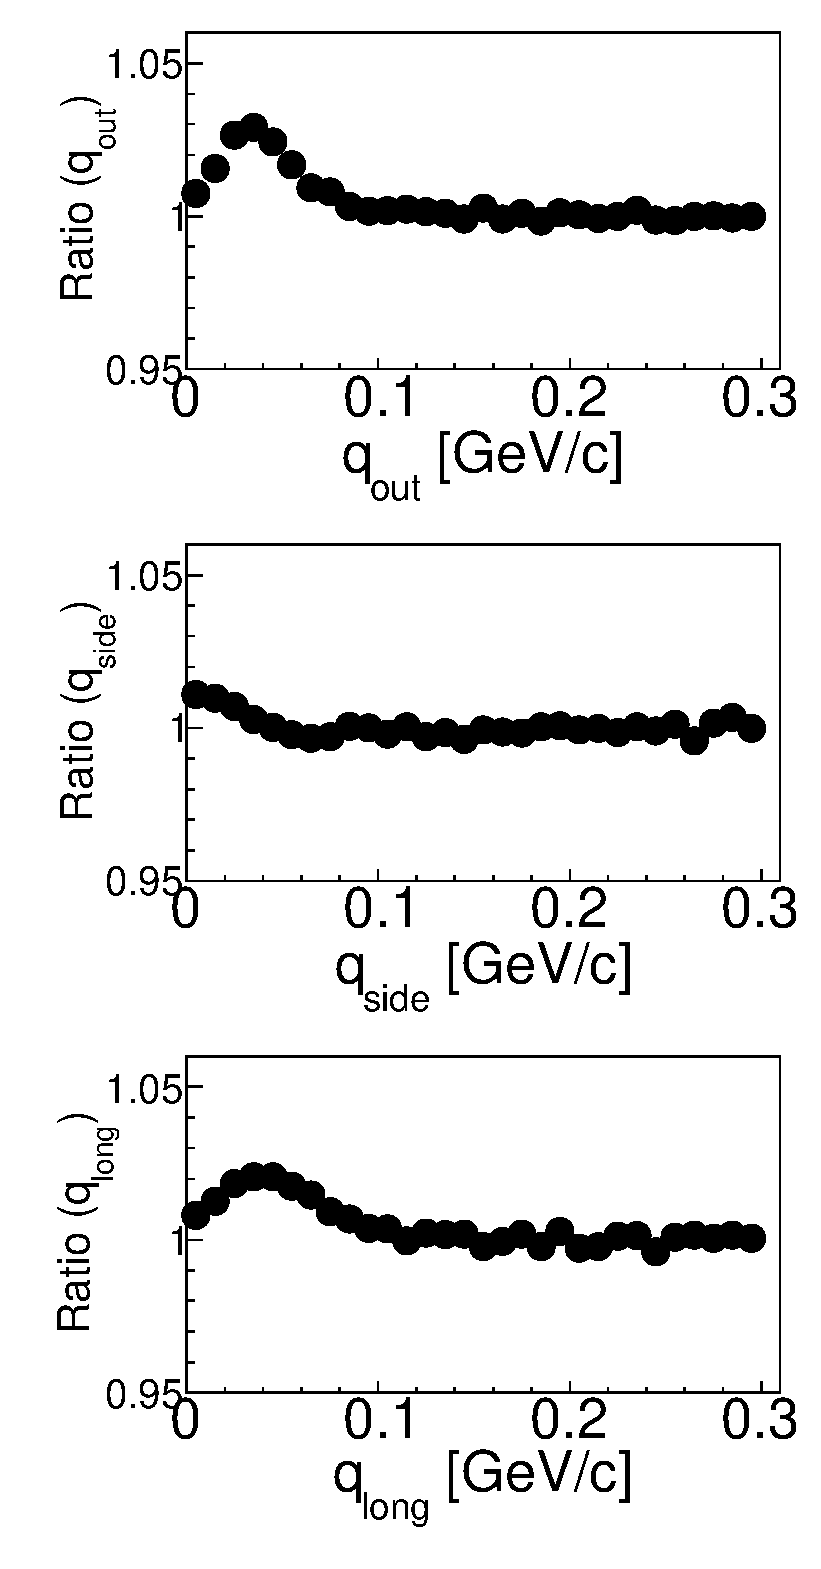
\includegraphics[width=0.99\linewidth]{fig3_poster.eps}
          \caption{Ratios of 1D projections of 3D correlation functions for the two EoS. 
     For each direction the corresponding ratio is calculated as follows: $C(q_{i}) (XPT) / C(q_{i}) (1PT)$, 
     where $i$ denotes ``out'', ``side'' and ``long'' directions, $1PT$ and $XPT$ denote a type of the used EoS.}
      \end{figure}
    \end{columns} 
   \end{block}
   
   \begin{figure}[H]
      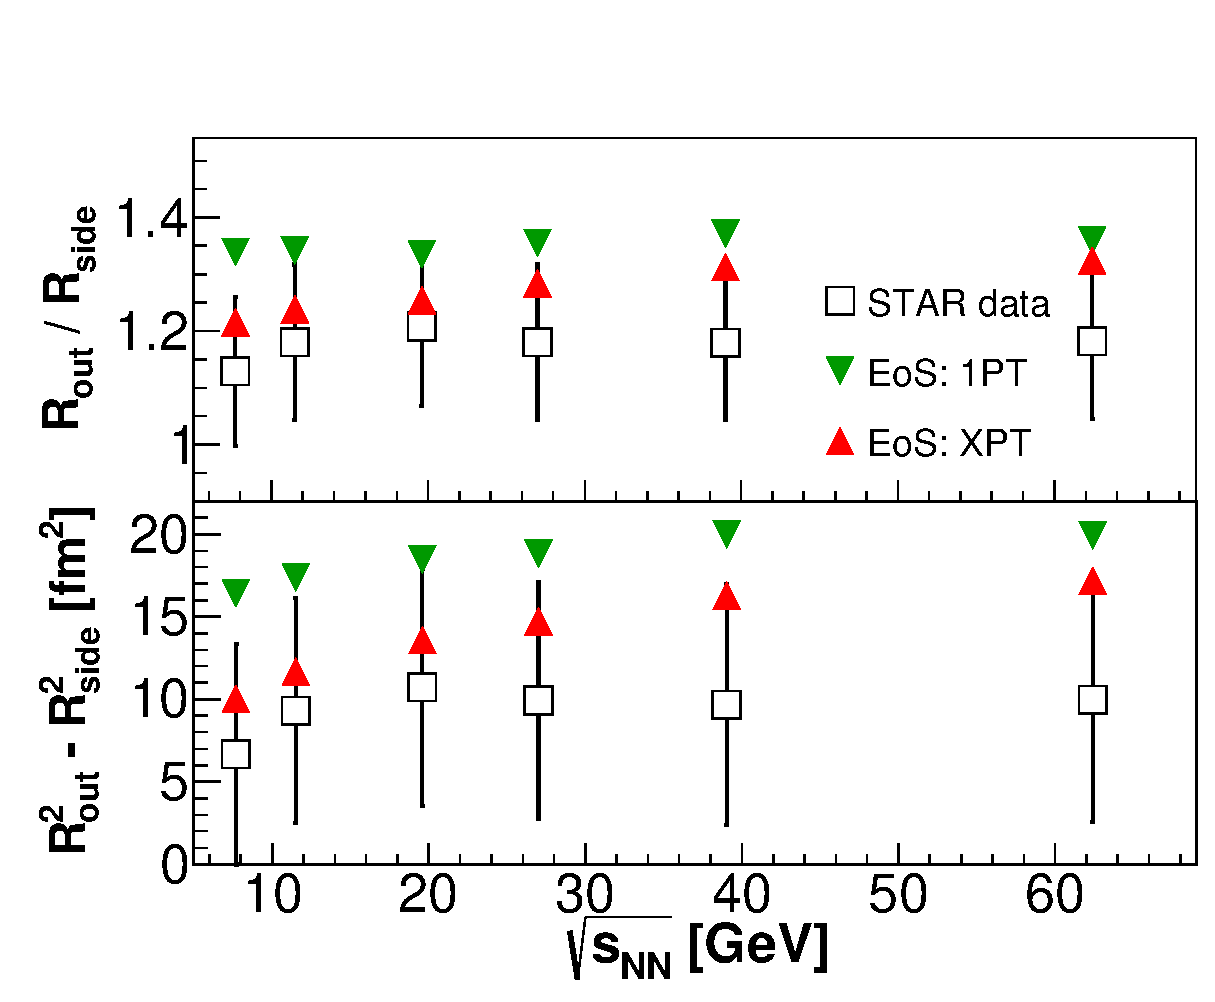
\includegraphics[width=1.\linewidth]{fig5_poster.eps}
      \caption{Ratio of the ``out'' and ``side'' radii (top) and difference of the radii squared (bottom) 
   as a function of $\sqrt{s_{NN}}$ derived from the STAR data ($0.15 < k_{T} < 0.25$ GeV/c, 0-5\% centrality) 
   and compared with the model calculations using the two EoS's.}
   \end{figure}
 

 \column{.53\textwidth}
 \begin{block}{vHLLE+UrQMD (Phys. Rev. C 91, 064901 (2015))}
  \begin{columns}[t]
  \column{.49\textwidth}
   \begin{figure}[t]
   \caption{Thermodynamic pressure as a function of energy density, 
   evaluated at zero baryon density from the equations of state used in the hydrodynamic stage: 
   chiral model EoS with crossover transition (XPT) and bag model EoS with first order phase transition (1PT).}
         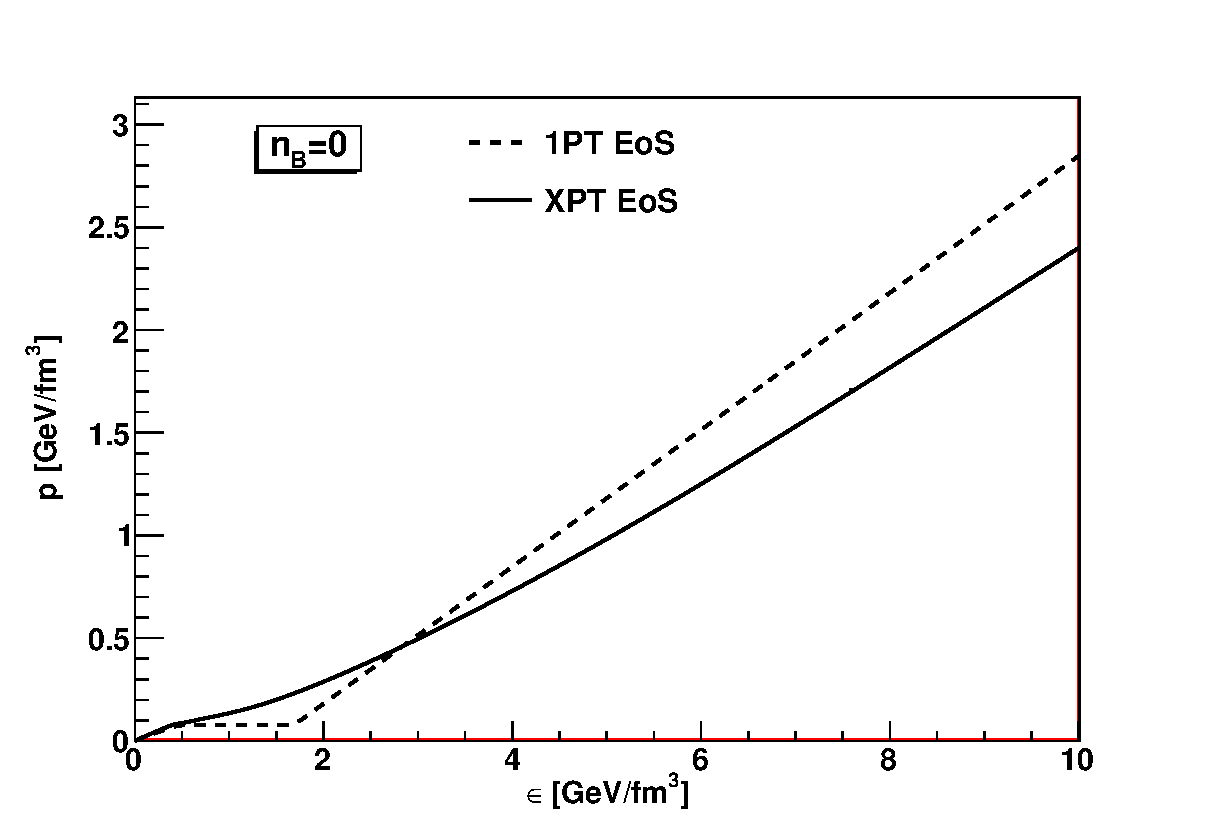
\includegraphics[width=1.01\linewidth]{eos.eps}
      \end{figure}
     
   \begin{table}
  \caption{Values of hydrodynamic starting time$\tau_0$, initial state granularity $R_\perp$, $R_\eta$ and shear viscosity over entropy ratio $\eta/s$ 
adjusted for different collision energies in order to reproduce basic observables in the RHIC BES region.} 
%An asterisk marks the values of $\tau_0$ which are adjusted instead of being set directly from Eq.~\ref{eqTau0}.}\label{tbParams}
\begin{tabular}{|l|l|l|l|l|}
\hline
 $\sqrt{s_{\rm NN}}$~[GeV] & $\tau_0$~[fm/c] & $R_\perp$~[fm] & $R_\eta$~[fm] & $\eta/s$ \\ \hline
     7.7          &      3.2        &     1.4        &     0.5    &    0.2   \\ \hline
     8.8 (SPS)    &      2.83       &     1.4        &     0.5    &    0.2   \\ \hline
     11.5         &      2.1        &     1.4        &     0.5    &    0.2   \\ \hline
     17.3 (SPS)   &      1.42       &     1.4        &     0.5    &    0.15  \\ \hline
     19.6         &      1.22       &     1.4        &     0.5    &    0.15  \\ \hline
     27           &      1.0        &     1.2        &     0.5    &    0.12  \\ \hline
     39           &      0.9        &     1.0        &     0.7    &    0.08  \\ \hline
     62.4         &      0.7        &     1.0        &     0.7    &    0.08  \\ \hline
     200          &      0.4        &     1.0        &     1.0    &    0.08  \\ \hline
 \end{tabular}
\end{table}  

\vskip 1.5cm 

\begin{block}{Tuning of the model}
Parameters of the model were adjusted basing on rapidity, transverse momentum spectra and elliptic flow data in the BES region for the XPT EoS scenario.

No readjustment for the 1PT EoS has been made.
\end{block}
      
  \column{.49\textwidth}
%% Table with params. of adjustment
  \begin{figure}[T]
   \caption{Pion emission times at the particlization surface (top) and the last interactions (bottom) in the center-of-mass system of colliding gold nuclei at different values of $\sqrt{s_{NN}}$.}
         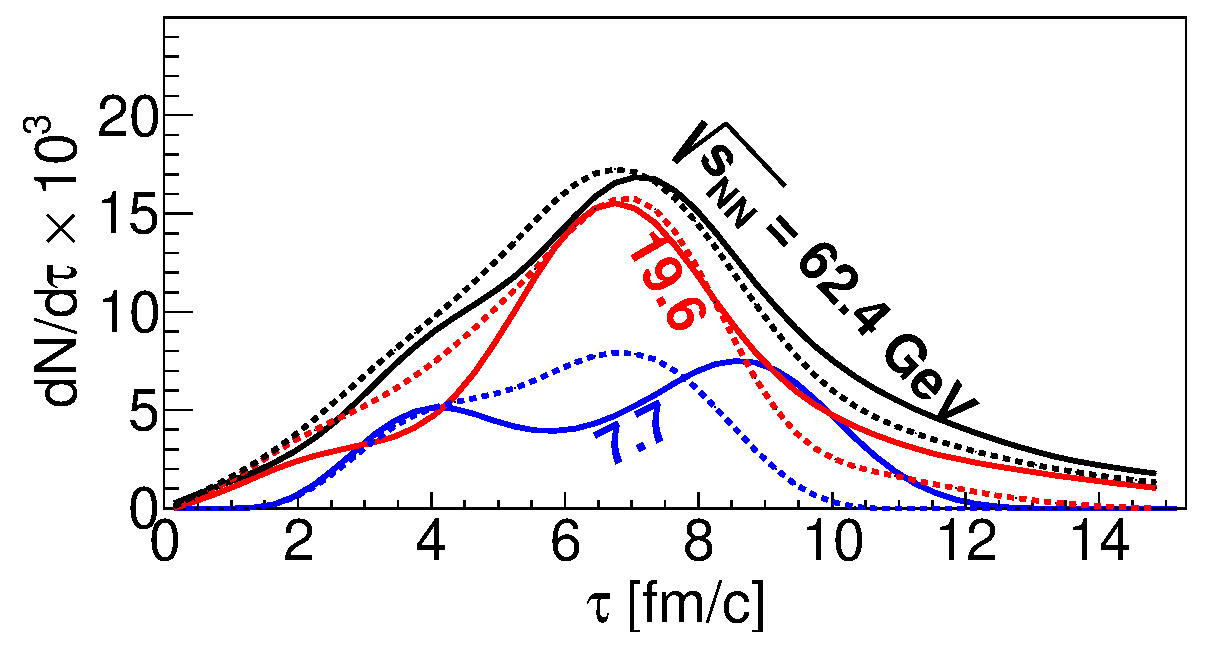
\includegraphics[width=1.\linewidth]{fig1b_poster.eps} \\
         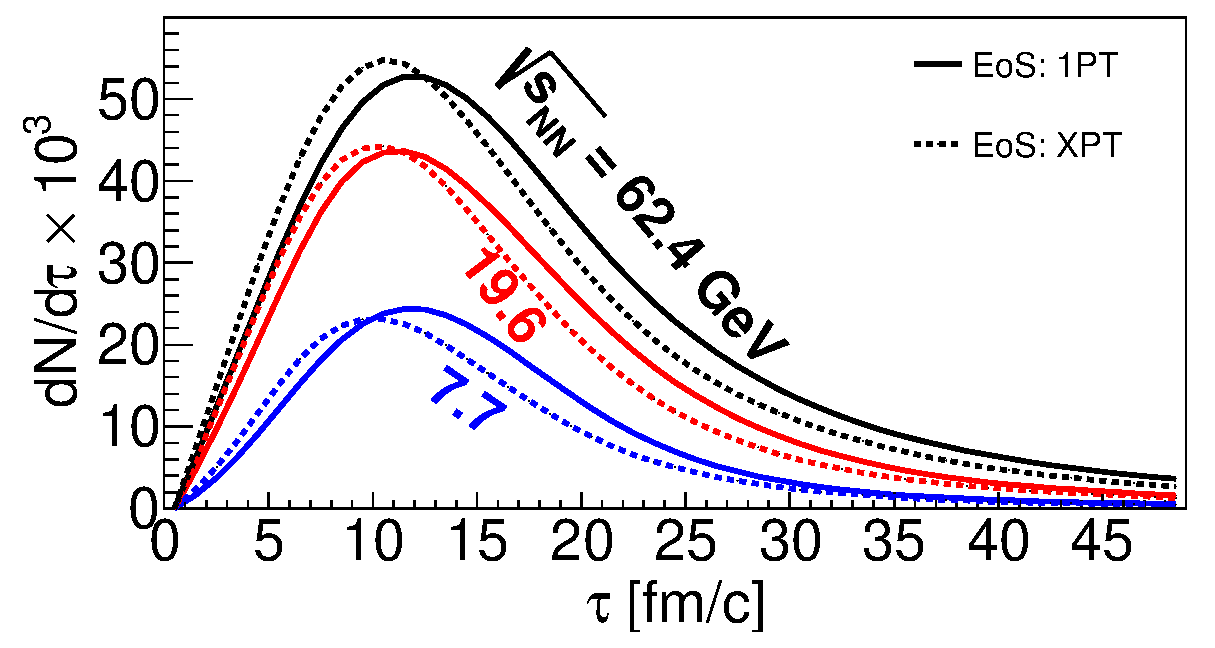
\includegraphics[width=1.\linewidth]{fig1a_poster.eps}
      \end{figure}

\begin{table}[!h]
\caption{Extracted average pion emission times $\bar{t}$ as a function of $\sqrt{s_{NN}}$ in the center-of-mass system of colliding gold nuclei depending on the EoS used.}
\begin{center}
\begin{tabular}{|c|c|c|c|c|c|}\hline
$\sqrt{s_{NN}}$ & \multirow{2}{*}{EoS} & \multicolumn{2}{c|}{particlization surface} & \multicolumn{2}{c|}{last interactions}\\
\cline{3-6} 
$[GeV]$& & $\bar{t}$ [fm/c] &  RMS [fm/c] & $\bar{t}$ [fm/c] & RMS [fm/c]\\
\hline
  \multirow{2}{*}{7.7}     & 1PT     &  7.24 & 2.84 & 13.15    & 6.56    \\
  & XPT   &  6.16 & 2.01 & 11.61    & 6.26 \\
\hline
  \multirow{2}{*}{11.5}       & 1PT     &  7.33 & 2.31 & 13.09    & 6.92    \\
  & XPT  &  6.36 & 1.91  & 11.57   & 6.41   \\
\hline
  \multirow{2}{*}{19.6}       & 1PT     & 6.88 & 2.16 & 13.18     &  7.56  \\
 & XPT  & 6.41 & 2.15 & 11.93    &    6.93  \\
\hline
  \multirow{2}{*}{27}       & 1PT     &   6.85 & 2.37 & 13.38   &  8.07  \\
   & XPT  &    6.40 & 2.39 & 12.62 &    7.57   \\
 \hline
 \multirow{2}{*}{39}        & 1PT     &   7.17 & 2.75 & 13.98   &  8.30   \\
   & XPT  &    6.64 & 2.58 & 13.05 &    7.85   \\
\hline
 \multirow{2}{*}{62.4}        & 1PT     &   7.00 & 2.82 & 14.11   &  8.50  \\
   & XPT  &    6.60 & 2.63 & 12.72 &    7.81 \\     
\hline
\end{tabular}
\end{center}
\end{table}
    
  \end{columns}
 \end{block} 
 
 \begin{block}{Extracted femtoscopic radii (Phys. Rev. C 92 014904 (2015))}
      \begin{figure}[H]
      \caption{Comparison of the 3D LCMS femtoscopy radii derived from the model 
      with those measured by the STAR collaboration at \newline $\sqrt{s_{NN}}$ = 7.7 - 62.4~GeV. Open squares represent the STAR data.}
         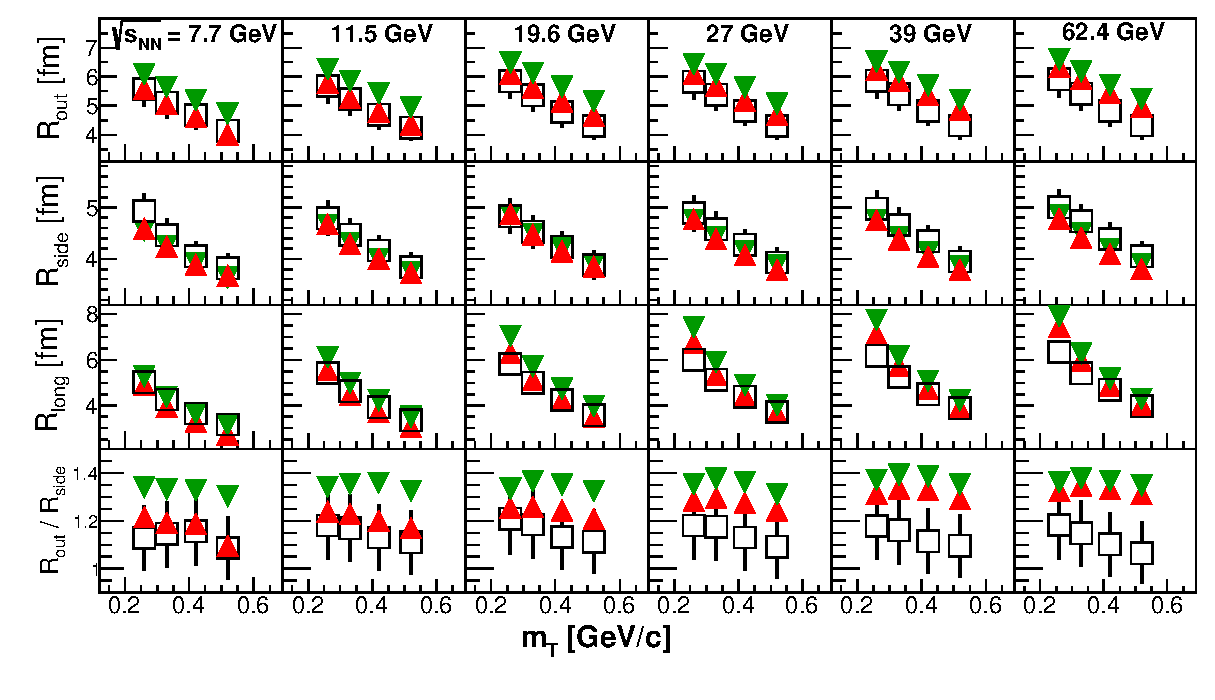
\includegraphics[width=1.0\linewidth]{fig4_poster.eps}
      \end{figure}
   \end{block}
   
 
   \begin{block}{Source emission functions}
     \begin{figure}[H]
 \caption{1D projections of source emission functions of pions 
 from the model obtained at $\sqrt{s_{NN}}$ = 7.7~GeV for pion pairs satisfying the cut on transverse momentum: 0.2$ < k_{T} < $0.4 GeV/c.}
         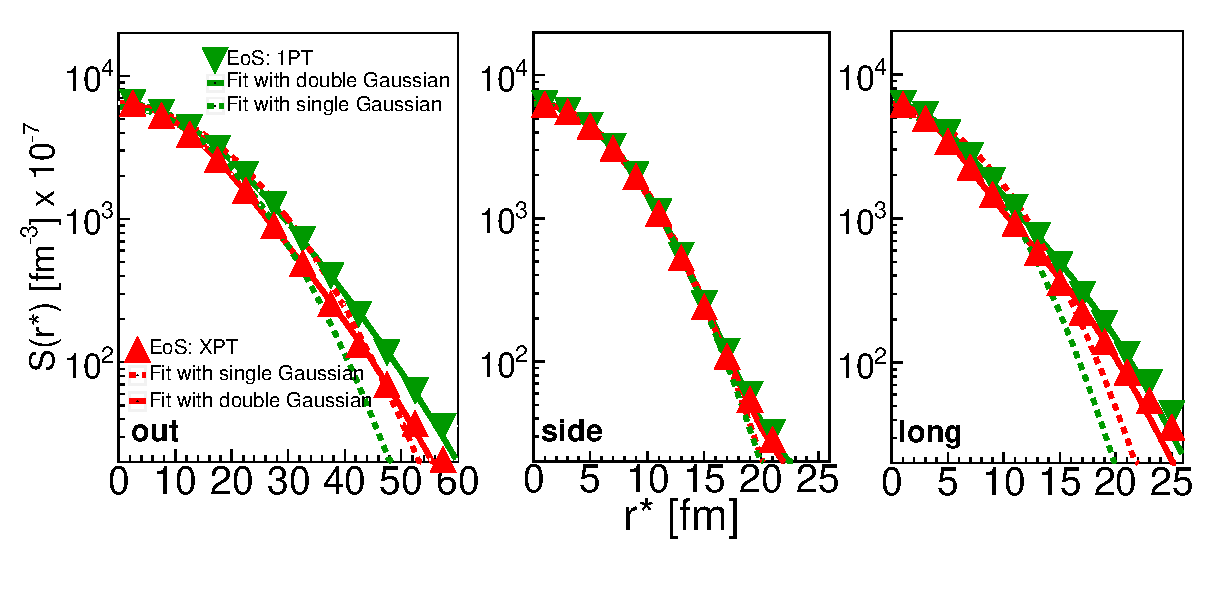
\includegraphics[width=1.\linewidth]{fig6_poster.eps}
 \end{figure}
 \end{block}
 
 \begin{block}{Conclusions:}
 {\small 
 %\begin{center}
 \begin{itemize}
  \item The chiral model EoS (XPT EoS), which has a crossover-type transition between QGP and hadron gas phases, in the fluid phase results in a quite reasonable reproduction of 3D pion femtoscopic radii measured by the STAR collaboration.
  \item The ``out'' Gaussian femtoscopic radii obtained with the bag model EoS (1PT EoS) are systematically larger as compared with the XPT EoS; the ``side'' radii coincide for both types of EoS; the ``long'' radii are also somewhat larger for the 1PT EoS.
  \item  No readjustment for the 1PT EoS poses an open question whether the differences in femtoscopic radii between the two EoS's will be even smaller if the readjustment is made for each EoS scenario individually. 
  \item No additional parameter tuning has been made for the femtoscopic observables, therefore the results may be considered as ``free model predictions'' even though the experimental data already exists.
  \item  A possibility to distinguish calculations with the two different EoS's using the source emission function technique has been shown. The projections of source emission functions onto ``out'' direction are wider for the use of the 1PT EoS. For ``side'' direction these projections coincide for both scenarios; for ``long'' direction the projections obtained with the 1PT EoS are also wider in comparison with calculations using the XPT EoS. This observation is related to a weaker transverse flow developed in the fluid phase and a longer lifetime of the phase in case of the 1PT EoS used.
  \item {\bf {\color{red} An attempt to perform similar calculations with Three-fluid Hydrodynamics-based Event Simulator Extended by UrQMD final State interactions (THESEUS)}\footnote{Phys. Rev. C94 (2016) 044917 (arXiv:1608.00965),  arXiv:1711.07959}  {\color {red} is planned to be done.}}
 \end{itemize}
 }
 %\end{center}
\end{block}
 
 \end{columns}
 \end{frame}
\end{document}
